\documentclass[crop,class=article]{standalone}
%----------------------------Preamble-------------------------------%
\usepackage{amsfonts}                   % Blackboard Bold R.
\usepackage{tikz}                       % Drawing/graphing tools.
\usetikzlibrary{arrows, arrows.meta}    % Latex/Open Interval arrow.
%--------------------------Main Document----------------------------%
\begin{document}
    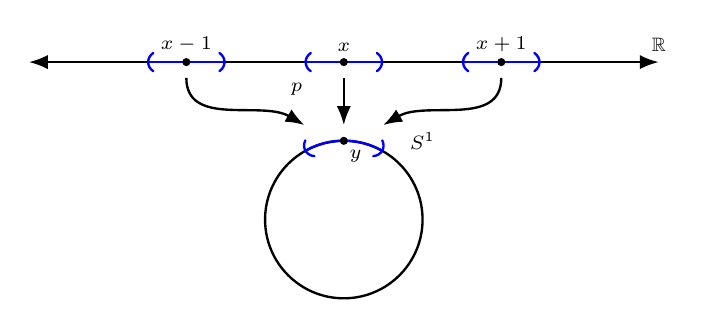
\begin{tikzpicture}[>=Latex,line width=0.3mm,font=\scriptsize]
        \draw[<->] (-4,0) to (4,0);
        \draw (0,-2) circle (1);
        \begin{scope}[(-),draw=blue]
            \draw (0.5,-1.13397) arc (60:120:1);
            \draw (-0.5,0) to (0.5,0);
            \draw (-2.5,0) to (-1.5,0);
            \draw (2.5,0) to (1.5,0);
        \end{scope}
        \begin{scope}[%
            every node/.style={
                circle,
                fill=black,
                draw=black,
                inner sep=0pt,
                minimum size=2pt
            }
        ]
            \node at (0,-1) {};
            \node at (0,0) {};
            \node at (-2,0) {};
            \node at (2,0) {};
        \end{scope}
        \draw[->]  (-2,-0.2) to [out=-90,in=150] (-0.5,-0.8);
        \draw[->]  (2,-0.2) to [out=-90,in=30] (0.5,-0.8);
        \draw[->] (0,-0.2) to (0,-0.8);
        \node at (-0.6,-0.35) {$p$};
        \node at (0.15,-1.2) {$y$};
        \node at (0,0) [above] {$x$};
        \node at (2,0) [above] {$x+1$};
        \node at (-2,0) [above] {$x-1$};
        \node at (4,0) [above] {$\mathbb{R}$};
        \node at (1,-1) {$S^{1}$};
    \end{tikzpicture}
\end{document}